\documentclass[10pt]{beamer}
\usepackage[latin1]{inputenc}
\usetheme{Warsaw}
\usecolortheme{orchid}
\usepackage{color}
%\usepackage{braket}
\usepackage{amsmath}
\usepackage{amsfonts}
\usepackage{amssymb}
\usepackage{graphicx}
%\setbeamerfont{page number in head/foot}{size=\normalsize}
%\setbeamertemplate{footline}[frame number]
\usepackage{ifthen}
\usepackage{animate}
\usepackage{movie15}
\usepackage{xmpmulti}

\newcommand*\oldmacro{}%
\let\oldmacro\insertshorttitle%
\renewcommand*\insertshorttitle{%
	\oldmacro\hfill%
	\insertframenumber\,/\,\inserttotalframenumber}
\setbeamercovered{invisible}
\usepackage{tikz}
\usetikzlibrary{calc}
\usepackage{pgfplots}
\usepackage{tikz-3dplot}
\usetikzlibrary{decorations.markings}
\usetikzlibrary{shapes,arrows}
\newcommand{\midarrowright}{\tikz \draw[-triangle 90] (0,0) -- +(.1,0);}
\newcommand{\midarrowup}{\tikz \draw[-triangle 90] (0,0) -- +(0,.1);}

\usetikzlibrary{shadings, calc, decorations.markings}
\tikzset{->-/.style={decoration={
			markings,
			mark=at position #1 with {\arrow{<}}},postaction={decorate}},
	->-/.default=0.3,
}

\tikzset{->>-/.style={decoration={
			markings,
			mark=at position #1 with {\arrow{<}}},postaction={decorate}},
	->>-/.default=0.7,
}

%\theoremstyle{definition}
%\newtheorem{definition}{Definition}

\theoremstyle{plain}
\newtheorem{prop}{Proposition}

\newcommand\ds{\displaystyle}
\newcommand\ts{\textstyle}
\newcommand{\mb}{\mathbf}
%\renewcommand{\thenotation}{}
%\renewcommand{\theequation}{\thesection.\arabic{equation}}
\def\Caption #1{\caption{\footnotesize #1}}
%\renewcommand\Caption{#1}{\Caption{\small{#1}}}
%\def\Caption #1{\Caption{\small{{#1}}}}

\def \Bfemph #1{\textbf{\emph{#1}}}


%\def\Proof.{{\medbreak\noindent{\it Dimostrazione}\enspace}}
\def\Proof{{\medbreak\noindent{\textbf{Proof.} }}}
\def\Proofsketch{{\medbreak\noindent{\textbf{Sketch of proof.} }}}
\def\endproof{~\hfill $\blacksquare$}
%\def\endproof{\hfill$\square$\par\medskip}

\def\Svolgimento{{\medbreak\noindent{\textit{Execution.} }}}
\def\Suggerimento{{\medbreak\noindent{\textit{Hint:} }}}


\def\mR{{\mathbb R}}
\def\mC{{\mathbb C}}
\newcommand{\parz}[2]{ \frac{\partial #1}{\partial #2}}
\newcommand{\deri}[2]{\displaystyle \frac{\dd #1}{\dd #2}}
\renewcommand{\Re}{\text{Re }}
\renewcommand{\Im}{\text{Im }}
%\renewcommand{\theta}{\vartheta}
\newcommand{\Int}{\text{Int }}
\newcommand{\Ext}{\text{Ext }}
\newcommand{\supp}{\text{supp}}
\newcommand{\mD}{\mathcal{D}}
\newcommand{\dd}{\mathrm d}
\newcommand{\norm}[1]{\displaystyle \left \| #1 \right \|}
\renewcommand{\div}{\operatorname{div}}
\newcommand{\rot}{\operatorname{rot}}
\newcommand{\grad}{\operatorname{grad}}
\newcommand{\id}{\mathds{1}}
\newcommand{\mM}{\mathrm{M}}
\newcommand{\mT}{\mathrm{T}}
%\renewcommand{\to}{\longrightarrow}
\newcommand{\scalar}[2]{\left\langle #1, #2 \right\rangle}
\newcommand{\mf}[1]{\mathbf{#1}}

\def\Xint#1{\mathchoice 
	{\XXint\displaystyle\textstyle{#1}}% 
	{\XXint\textstyle\scriptstyle{#1}}% 
	{\XXint\scriptstyle\scriptscriptstyle{#1}}% 
	{\XXint\scriptscriptstyle\scriptscriptstyle{#1}}% 
	\!\int} 
\def\XXint#1#2#3{{\setbox0=\hbox{$#1{#2#3}{\int}$} 
		\vcenter{\hbox{$#2#3$}}\kern-.5\wd0}} 
\def\Mint{\Xint -}


\renewcommand{\hat}[1]{\widehat{#1}}
\renewcommand{\theta}{\vartheta}
\renewcommand{\epsilon}{\varepsilon}
%\renewcommand{\phi}{\varphi}
\newcommand{\res}{\mathop{\mathrm{Res }}}

\newcommand{\colonna}[2]{\begin{pmatrix}
		#1 \\ #2
\end{pmatrix}}
\newcommand{\riga}[2]{\begin{pmatrix}
		#1 & #2
\end{pmatrix}}
%%%%%%%%%%%%%%%%%%%%%%%%%%%%%%%%%%%%%%%%%%%%%%%%%%%%%%%%%%%%%%%%%%%%%%%%%%%%%%%%%%%%%%%%%%%

\newcounter{angle}
\setcounter{angle}{0}

\title{Introduction to Quantum Backflow}
\author{Eugenio Mauri}
\date

\begin{document}
	
	\begin{frame}
		\maketitle
		\footnotesize Supervisor: Prof. Claudio Dappiaggi\\
		Co-supervisor: Dr. Nicol\`{o} Drago.
	\end{frame}
	
%	\section{Introduction}
	\begin{frame}
		\frametitle{What Quantum Backflow is?}
		\textbf{Setting}: Consider a non-relativistic \alert<1>{free particle} in one dimension\pause
		\begin{itemize}
			\item Suppose that at time $t=0$ the particle has \alert<2>{positive momentum} with probability $1$.\pause
			\item Consider the probability $P(t)$ of finding the particle at $x<0$ at time $t$. What is the \alert<3>{time-dependence} of $P(t)$?
		\end{itemize}\pause
		Answers:
		\begin{itemize}
			\item[-] In \alert{classical physics}: $P(t)$ is always decreasing in time.\pause
			\item[-] In \alert{quantum physics}: not necessarily.
		\end{itemize}
	\end{frame}
	
	\begin{frame}
				\frametitle{What Quantum Backflow is?}
		\multiinclude[format=png, start=1,graphics={scale=0.5}]{../images/gand}
	\end{frame}
	
	\begin{frame}
				\frametitle{What Quantum Backflow is?}
		\centering
		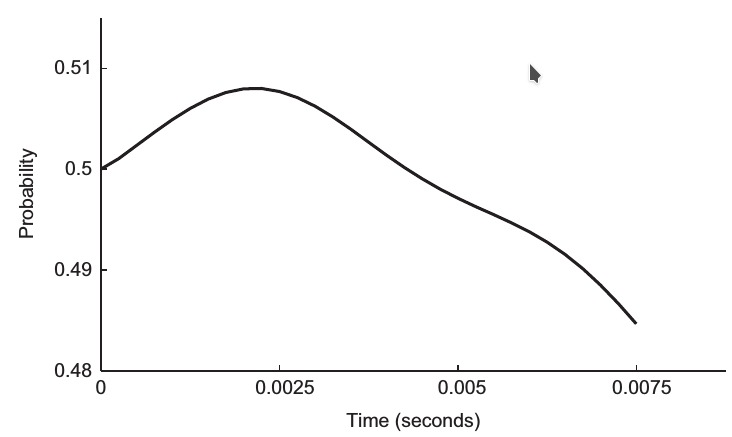
\includegraphics[scale=0.4]{../images/P(T)}
	\end{frame}
%	\section{Backflow in Free Theory}
	\begin{frame}
		\frametitle{Right-movers}
		What does it means that a particle \textquotedblleft travels to the right\textquotedblright?\pause
		\begin{definition}
			Let $\psi\in L^2(\mR)$ be a wave-function associated to a single particle.  We call $\psi$ a \alert<2>{\textbf{right-mover}} if $\mathrm{supp}\ \hat{\psi}\in[0,+\infty)$.
		\end{definition}\pause
		\begin{definition}
			We call $E_\pm:L^2(\mR)\to L^2(\mR)$ the operator such that:
			\begin{equation*}
			\mathcal{F}[E_\pm\psi](p)=\theta(\pm p)\hat{\psi}(p)\ \forall \psi\in L^2(\mR),
			\end{equation*}
			where $\theta$ is the Heaviside function.
		\end{definition}
		$E_+$ projects into the space of right-movers.
	\end{frame}
	
	\begin{frame}
		\frametitle{Temporal boundedness of backflow}
		\begin{itemize}
			\item[-] Consider $L(\psi_T)=\int_{0}^{\infty}\!\!|\psi_T(x)|^2\,\dd x$. \medskip \pause
			\item[-] Searching for the \alert<2>{maximum} amount of backflow:\\			
				$\lambda=\sup\{L(\psi_0)-L(\psi_T)\ |\ \|\psi\|=1,\ E_+\psi=\psi,\ T>0 \}$
		\medskip 	\pause
			\item[-] Using scaling arguments, it holds\\ $\lambda=\sup\{L(\psi_0)-L(\psi_1)\ |\ \|\psi\|=1,\ E_+\psi=\psi\}$\pause
		\end{itemize}
	\begin{prop}
		Let $K:L^2(\mR_+)\to L^2(\mR_+)$ be the integral operator:
		\begin{equation*}
		(Kf)(u)=-\frac{1}{\pi}\int_{0}^{\infty}\frac{\sin(u^2-v^2)}{u-v}f(v)\, \dd v \ \ \forall f\in L^2(\mR_+).
		\end{equation*}
		Then $K$ is \alert{bounded} and \alert{self-adjoint}, and \alert{$\lambda=\sup \sigma(K)$}.
	\end{prop}
	In fact, it holds $L(\psi_{-1})-L(\psi_1)=(\psi|K\psi)$ with $\psi=E_+\psi$.\\ %\textcolor[rgb]{0,0,.7}{\textsc{[Bracken, Melloy]}}
		
	\end{frame}
	
	\begin{frame}
		\frametitle{Temporal boundedness of backflow}
		\begin{theorem}[\textbf{Temporal boundedness of backflow}]
			Let $\lambda=\sup \sigma(K)$. For any right-mover $\psi\in L^2(\mR)$ such that $\psi=E_+\psi$ and for any $T>0$ it holds 
			\begin{equation*}
			\int_{0}^{T}\!\!\!\!j_\psi(0,t)\, \dd t\ge -\lambda>-\infty.
			\end{equation*}
		\end{theorem}\pause
		\Proofsketch Since $K$ is bounded and self-adjoint, it holds $\sigma(K)\subseteq [-\|K\|,\|K\|]$. \endproof \pause\\ \bigskip
		How to evaluate $\lambda$? Using numerical methods\footnote<3->{M. Penz, G. Gr�bl, S. Kreidl and P. Wagner, \textit{A new approach to quantum
			backflow}, J. Phys. A: Math. Gen. \textbf{39}, 2005. }.
	\end{frame}
	
	\begin{frame}
		\begin{figure}[h]	
			\centering
			\begin{minipage}{0.45\textwidth}
				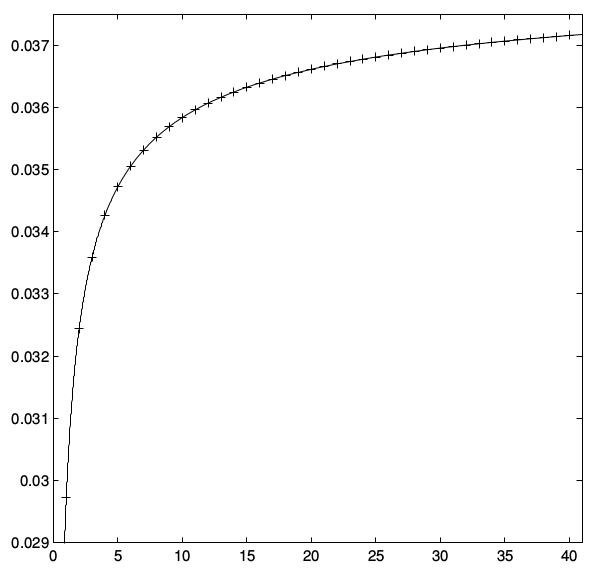
\includegraphics[scale=0.25]{../images/backflow_approx_1}
				%\caption{$\lambda$ plotted against $h$ and fit $\lambda_\infty+b/\sqrt h$.}
				%\label{fig:backflow_approx_1}
			\end{minipage}
			\hfil
			\begin{minipage}{0.45\textwidth}
				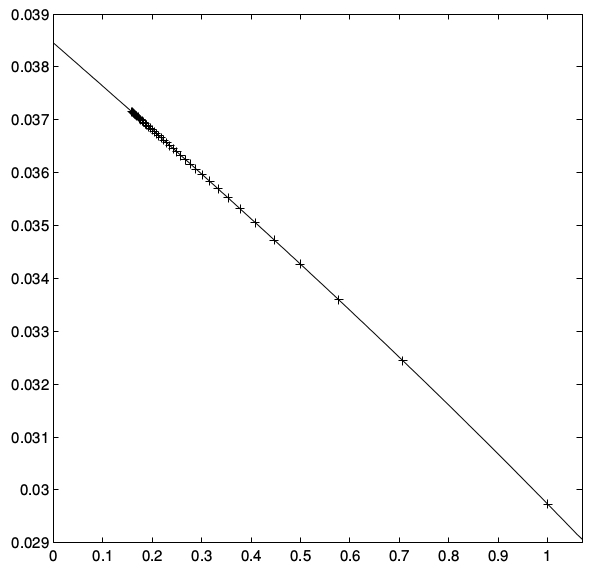
\includegraphics[scale=0.25]{../images/backflow_approx_2}
				%\caption{$\lambda$ plotted against $1/\sqrt h$ and polynomial fit of third order.}
				%\label{fig:backflow_approx_2}
			\end{minipage}
		\end{figure}
		\begin{center}
			\Large $\lambda\approx0.0384517$
		\end{center} 
	\end{frame}
	
	\begin{frame}
		\frametitle{Spatial extension of Backflow}
		What about the spatial properties of backflow?\pause 
		\begin{block}{Lemma}
			There exist sequences of normalized right-movers $\phi_n^\pm\in E_+(L^2(\mR))$ such that $ \lim_{n\to\infty}j_{\phi_n^\pm}(x)=\pm\infty$.
		\end{block}\pause
		\textbf{NB}: Unboundedness from below as \alert<3>{superposition of high and low momenta}.\\ \medskip \pause
		Consider the integral, with test functions $f$, $\int_{\mR}f(x)j_\psi(x)\,\dd x\equiv (\psi|J(f)\psi)$.\\
		$J(f)$ exists as operator.\pause
		\begin{prop}
			For any $f\in \mathcal{S}(\mR)$, $f\ge0$, there exists a constant $\beta_0(f)\in(-\infty,0)$ such that $(\psi|E_+J(f)E_+\psi)\ge\beta_0(f)$.
		\end{prop}
		
	\end{frame}
	
%	\section{Backflow in Scattering Theory}
	\begin{frame}
		\frametitle{Asymptotic right-movers}
		Consider an \alert<1>{interacting} system with Hamiltonian $H=H_0+V$.\pause
		\begin{itemize}
			\item[-] The time evolution $e^{-iHt}$ \alert<2>{does not preserve} the space of right-movers $E_+(L^2(\mR))$.\pause
			\item[-] \alert<3>{Reflection} may destroy backflow.\pause
		\end{itemize}
		Consider \alert<4-5>{asymptotic right-moving} states and the \alert<4-5>{M\o{}ller operator}:\pause
		\begin{equation*}
		\Omega_V:=\lim_{t\to-\infty}e^{itH}e^{-itH_0}
		\end{equation*}\pause
		\begin{itemize}
			\item[-] \footnote<6->{D. R. Yafaev, \textit{Mathematical Scattering Theory}: Analytic Theory, Mathematical
				Surveys and Monographs Vol. 158, American Mathematical Society, Providence,
				RI, 2010.}exists under regularity and short-range assumptions on $V$.\pause
			\item[-] links \textquotedblleft free\textquotedblright  solutions of Schr\"{o}dinger equation with \textquotedblleft interacting" ones.
		\end{itemize}
	\end{frame}
	
	\begin{frame}
		\frametitle{Asymptotic right-movers}
		\begin{definition}
			Let $V\in L^1(\mR)$ be a potential. We call $V$ as a \textquotedblleft short-range"  potential (indicated $V\in L^{1+}(\mR)$) if it satisfies\\ \centering $\|V\|_{1+}=\int_{\mR}\!\dd x\,(1+|x|)|V(x)|<+\infty$.
		\end{definition}\pause
		\begin{theorem}
			Let $V\in L^{1+}(\mR)$. Then
			\begin{itemize}
				\item[(a)] $\Omega_V$ exists.
				\item[(b)] $[-\partial_x^2+2V(x)-k^2]\psi(x)=0$ has unique solutions
				\begin{equation*}
				\varphi_k(x)=\begin{cases}
				T_V(k)e^{ikx}+o(1) & \text{for }  x\to+\infty\\
				e^{ikx}+R_V(k)e^{-ikx}+o(1) & \text{for } x\to-\infty
				\end{cases}
				\end{equation*}
				\item[(c)] For any $\hat{\psi}\in C_0^\infty(\mR)$, $(\Omega_VE_+\psi)(x)=\frac{1}{\sqrt{2\pi}}\int_{0}^{\infty}\!\varphi_k(x)\hat{\psi}(k)\, \dd k.$
			\end{itemize}
		\end{theorem}
	\end{frame}
	
	\begin{frame}
		\frametitle{Backflow and Scattering}
		We search bounds for the \alert{averaged current}, $f\ge0$\pause
		\begin{equation*}
		\int_{\mR}f(x)j_{\Omega_VE_+\psi}(x)\, \dd x=(\psi|E_+\Omega_V^*J(f)\Omega_VE_+\psi).
		\end{equation*}\pause
		Expanding $E_+\Omega_V^*J(f)\Omega_VE_+$ it holds\footnote<3->{H. Bostelmann, D. Cadamuro, G. Lechner, \textit{Quantum backflow and scattering},
			Physical Review A. \textbf{96}, 2017.}
		\begin{equation*}
		(\psi|E_+\Omega_V^*J(f)\Omega_VE_+\psi)\ge \beta_0(f)-2\alert<4>{\|J(f)(i+P)^{-1}\|}[2+\alert<5>{\|P(\Omega_V-T_V)E_+\|}].
		\end{equation*}\pause
		It descends $\alert<4>{\|J(f)(i+P)^{-1}\|}\le\|f\|_{\infty}+\frac{1}{2}\|f'\|_{\infty}$.\pause
		\begin{block}{Lemma}
			Let $V\in L^{1+}(\mR)$. Then, there exists $c_V\in\mR$ such that
			\begin{equation*}
			\alert<5>{\|P(\Omega_V-T_V)E_+\|\le 2c_V\|V\|_{1+}}
			\end{equation*}
		\end{block}
	\end{frame}
	
%	\begin{frame}
%		\frametitle{Backflow and Scattering}
%		\begin{block}{Lemma}
%			Let $V\in L^{1+}(\mR)$. Then, there exists $c_V\in\mR$ such that
%			\begin{equation*}
%			\|P(\Omega_V-T_V)E_+\|\le 2c_V\|V\|_{1+}
%			\end{equation*}
%		\end{block}\pause
%		\Proofsketch Rewrite the time-independent Schr\"{o}dinger equation as (Lippman-Schwinger equation)
%		\begin{equation*}
%		\varphi_k(x)=T_V(k)e^{ikx}+\int_{-\infty}^{\infty}\! 2V(y)G_k(y-x)\varphi_k(y)\, \dd y,
%		\end{equation*}
%		where $G_k(x)=\sin(kx)\theta(x)/k$\pause, and estimate 
%		\begin{equation*}
%		(P(\Omega_V-T_V)E_+\psi)(x)=\frac{-i}{\sqrt{2\pi}}\frac{\dd}{\dd x}\int_{0}^{\infty}\!\!\!\!\!\dd k\int_\mR\!\! \dd y\, V(y)G_k(x-y)\varphi_k(y)\tilde{\psi}(k)
%		\end{equation*}
%		with the known asymptotics for $\varphi_k(x)$
%	\end{frame}
	
	\begin{frame}
		\frametitle{Backflow and Scattering}
		\begin{theorem}[\textbf{Boundedness of Backflow in scattering scenarios}]
			For any potential $V\in L^{1+}(\mR)$ and for any non-negative $f\in\mathcal{S}(\mR)$, there exists a constant $\beta_V(f)\in(-\infty,0)$ such that
			\begin{equation*}
			(\psi|E_+\Omega_V^*J(f)\Omega_VE_+\psi)\ge\beta_V(f)\ \forall\ \psi\in L^2(\mR).
			\end{equation*}
		\end{theorem}\pause
		\begin{itemize}
			\item[-] Reflection \alert<2>{does not destroy} boundedness of backflow.\smallskip\pause
			\item[-] Heuristic explanation: Backflow is a \alert<3>{high momentum effect}, but for but for high momentum, reflection
			processes are suppressed sufficiently well. \smallskip\pause
			\item[-] What about \alert<4>{experimental} observations? (Bose-Einstein condensate, Bragg pulse, superposition of different momentum sates...)\footnote<4->{M. Palmero, E. Torrontegui, J. G. Muga, and M. Modugno, Phys. Rev. A \textbf{87}, 2013.}
		\end{itemize}
	\end{frame}
	
	\begin{frame}
		\frametitle{Conclusions}
		\begin{itemize}
			\item Backflow in Free Theory:\smallskip
			\begin{itemize}
				\item[-] Independence from time\smallskip
				\item[-] Existence of maximum backflow $\lambda\approx0.0038$\smallskip
				\item[-] Bound for spatially averaged backflow
			\end{itemize}\medskip
			\item Backflow in Scattering Theory
			\begin{itemize}
				\item[-] Asymptotic right-movers and M\o{}ller operator\smallskip
				\item[-] Existence of backflow in scattering scenarios\smallskip
				\item[-] Boundedness of backflow in scattering scenarios
			\end{itemize}
		\end{itemize}
	\end{frame}
	
	\begin{frame}[noframenumbering]
		\frametitle{Appendix: Experimental set-up}
		\begin{figure}
			\centering
			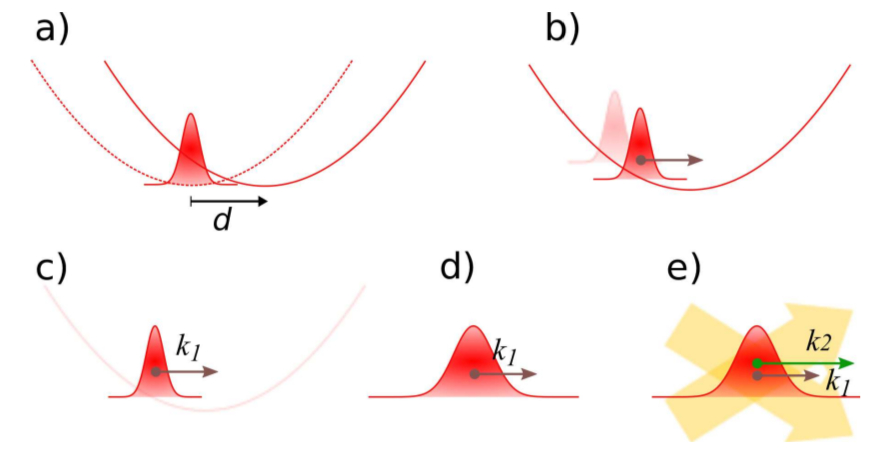
\includegraphics[scale=0.3]{../images/bose}
		\end{figure}
		
	\end{frame}
	
	
\end{document}
